% Copyright (c) 2009-2012 by the University of Waikato, Hamilton, NZ. 
% This work is made available under the terms of the 
% Creative Commons Attribution-ShareAlike 3.0 license, 
% http://creativecommons.org/licenses/by-sa/3.0/. 
%
% Version: $Revision: 4279 $

\documentclass[a4paper]{book}

\usepackage{wrapfig}
\usepackage{graphicx}
\usepackage{hyperref}
\usepackage{multirow}
\usepackage{scalefnt}
\usepackage{tikz}

% watermark -- for draft stage
\usepackage[firstpage]{draftwatermark}
\SetWatermarkLightness{0.9}
\SetWatermarkScale{5}

% Copyright (c) 2009 by the University of Waikato, Hamilton, NZ. 
% This work is made available under the terms of the 
% Creative Commons Attribution-ShareAlike 3.0 license, 
% http://creativecommons.org/licenses/by-sa/3.0/. 
%
% Version: $Revision$

\newenvironment{tight_itemize}{
\begin{itemize}
  \setlength{\itemsep}{1pt}
  \setlength{\parskip}{0pt}
  \setlength{\parsep}{0pt}}{\end{itemize}
}

\newenvironment{tight_enumerate}{
\begin{enumerate}
  \setlength{\itemsep}{1pt}
  \setlength{\parskip}{0pt}
  \setlength{\parsep}{0pt}}{\end{enumerate}
}

% if you just need a simple heading
% Usage:
%   \heading{the text of the heading}
\newcommand{\heading}[1]{
  \vspace{0.3cm} \noindent \textbf{#1} \newline
}

\newcommand{\icon}[1]{\tikz[baseline=-3pt]\node[inner sep=0pt,outer sep=0pt]{\includegraphics[height=1.1em]{#1}};}


\title{
  \textbf{ADAMS} \\
  {\Large \textbf{A}dvanced \textbf{D}ata mining \textbf{A}nd \textbf{M}achine
  learning \textbf{S}ystem} \\
  {\Large Module: adams-gnuplot} \\
  \vspace{1cm}
  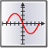
\includegraphics[width=2cm]{images/gnuplot-module.png} \\
}
\author{
  Peter Reutemann
}

\setcounter{secnumdepth}{3}
\setcounter{tocdepth}{3}

\begin{document}

\begin{titlepage}
\maketitle

\thispagestyle{empty}
\center
\begin{table}[b]
	\begin{tabular}{c l l}
		\parbox[c][2cm]{2cm}{\copyright 2009-2013} &
		\parbox[c][2cm]{5cm}{
\includegraphics[width=5cm]{images/coat_of_arms.pdf}} \\
	\end{tabular}
	
\includegraphics[width=12cm]{images/cc.png} \\
\end{table}

\end{titlepage}

\tableofcontents
\listoffigures
%\listoftables

%%%%%%%%%%%%%%%%%%%%%%%%%%%%%%%%%%%
\chapter{Introduction}
Gnuplot\cite{gnuplot} is an extremely
versatile command-line plotting tool, that allows you to plot all kinds of
graphs (e.g., plots with error bars, surface plots, plotting formulas). It
has been under development since 1986 and is also used in popular scientific
software like GNU Octave\footnote{\url{http://www.gnu.org/software/octave/}{}}.

ADAMS offers you tools for turning data into Gnuplot data and script files, 
allowing you to take advantage of its advanced visualization techniques.

\begin{figure}[htb]
  \begin{minipage}[b]{0.5\linewidth}
  \centering
  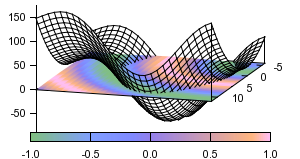
\includegraphics[width=4cm]{images/example_plot1.png}
  \caption{Surface plot.}
  \label{example_plot1}
  \end{minipage}%
  \begin{minipage}[b]{0.5\linewidth}
  \centering
  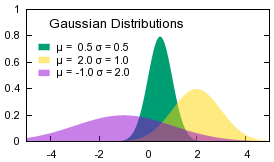
\includegraphics[width=4cm]{images/example_plot2.png}
  \caption{Gaussian distributions.}
  \label{example_plot2}
  \end{minipage}
\end{figure}

% %%%%%%%%%%%%%%%%%%%%%%%%%%%%%%%%%%
\chapter{Generating output}
ADAMS offers you Gnuplot support for outputting the data in Gnuplot format
and also generating scripts for plotting the data. The following sections
explain this in more detail.

\section{Data}
The most important step is to get the data from ADAMS into a format that 
Gnuplot can handle. Any data that is in spreadsheet format, can be output
using the \textit{SpreadSheetWriter} sink in conjunction with the 
\textit{GnuplotSpreadSheetWriter} writer. Figure \ref{write_data_file-flow} shows
a very simple flow\footnote{adams-gnuplot-create\_data\_file.flow} that dumps
the spreadsheet data obtained from a CSV (comma-separated values) files as
Gnuplot data file. This file can be plotted using the Gnuplot command-line
interface. The raw data file is shown in Figure \ref{write_data_file-output}.

\begin{figure}[htb]
  \centering
  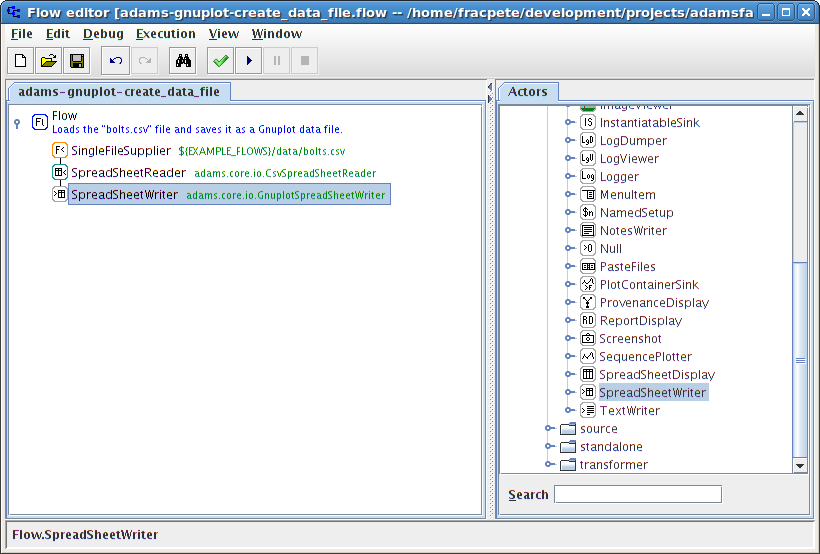
\includegraphics[width=10.0cm]{images/write_data_file-flow.png}
  \caption{Flow for outputting spreadsheet data in Gnuplot format.}
  \label{write_data_file-flow}
\end{figure}

\begin{figure}[htb]
  \centering
  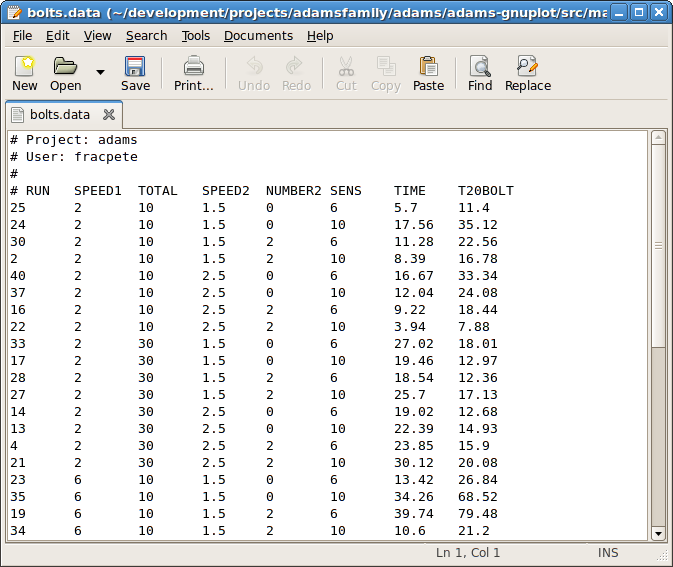
\includegraphics[width=10.0cm]{images/write_data_file-output.png}
  \caption{The generated Gnuplot data file.}
  \label{write_data_file-output}
\end{figure}

\clearpage
\newpage
\section{Scripts}
Outputting the spreadsheet data as Gnuplot data file is only the first step
and only recommended if you already have an existing script for plotting the
data. With ADAMS, you can also automate the process of generating a file 
containing the commands for plotting the data. The \textit{GnuplotScript}
sink can be used to generate a script file for plotting the data.

ADAMS offers already some basic scriptlets for generating parts of the script
file:
\begin{tight_itemize}
	\item \textit{Initialize} -- Initializes the plot, e.g., sets plot and 
	axes titles, output terminal.
	\item \textit{CustomScriptlet} -- Use this ``free text'' scriptlet if you 
	need more advanced plotting features that the other scriptlets don't offer.
	\item \textit{MultiScriptlet} -- Groups multiple scriptlets and combines
	the output of all of them.
	\item \textit{Pause} -- Adds a ``pause'' statement to the flow, usually
	used as last scriplet.
	\item \textit{SimplePlot} -- Allows you to plot several columns as 
	predefined plot types (points, lines, error plots, \ldots).
\end{tight_itemize}
In Figure \ref{command-lines} you can see the command-lines of all the 
scriptlets that are used in Figures \ref{write_data_and_script-flow} 
and \ref{write_data_and_script-output}. Here a dataset for supervised
learning is used to plot two attributes versus the class 
attribute.\footnote{adams-gnuplot-generate\_gnuplot\_script.flow}

\begin{figure}[htb]
{\scriptsize
\begin{verbatim}
adams.core.gnuplot.Initialize -title "bolts dataset" -x-label "target variable" -y-label "input variables"
adams.core.gnuplot.SimplePlot -cols 8:2 -plot-type POINTS -plot-name "speed1 vs t20bolt" -first-plot
adams.core.gnuplot.SimplePlot -cols 8:7 -plot-type POINTS -plot-name "time vs t20bolt"
adams.core.gnuplot.Pause -waiting-period 5 -message "Press <Enter> to close the plot..."
\end{verbatim}
}
  \caption{Command-lines of example scriptlets for plotting data.}
  \label{command-lines}
\end{figure}

\begin{figure}[htb]
  \centering
  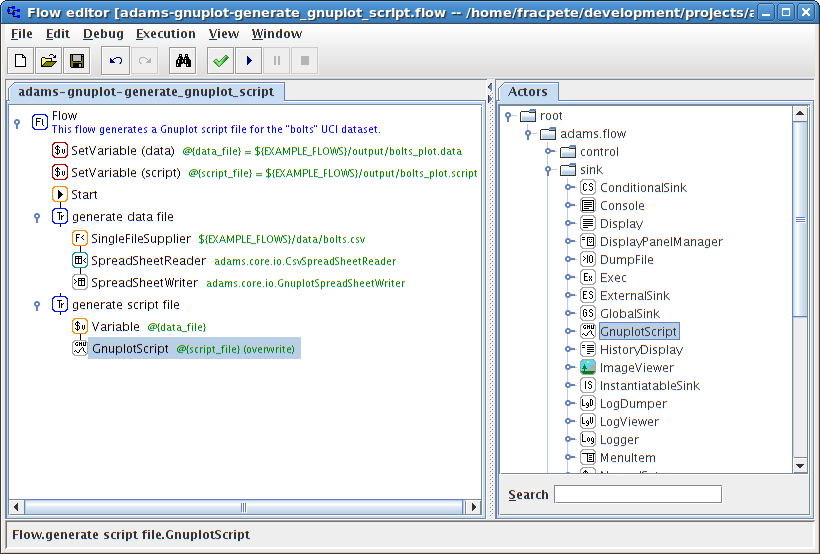
\includegraphics[width=10.0cm]{images/write_data_and_script-flow.png}
  \caption{Flow for outputting spreadsheet data in Gnuplot format and 
  generating a script for plotting it.}
  \label{write_data_and_script-flow}
\end{figure}

\begin{figure}[htb]
  \centering
  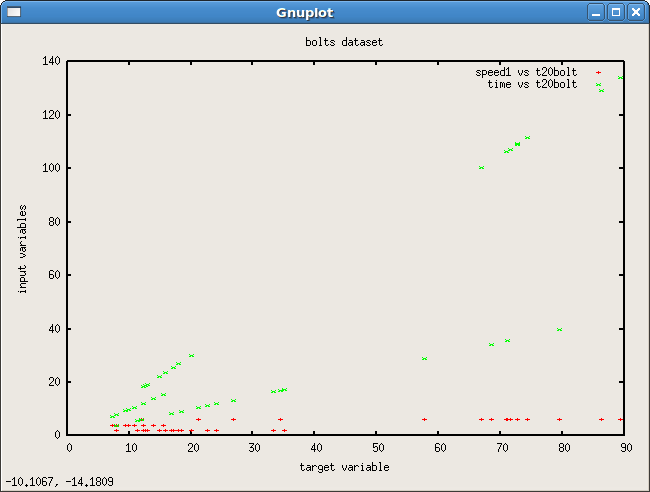
\includegraphics[width=10.0cm]{images/write_data_and_script-output.png}
  \caption{The generated plot.}
  \label{write_data_and_script-output}
\end{figure}


%%%%%%%%%%%%%%%%%%%%%%%%%%%%%%%%%%%
\chapter{Running gnuplot}
Simply generating the data and script files might not be sufficient in all
circumstances, but executing the script itself can be necessary. Using the 
\textit{Gnuplot} standalone, you can simply execute any script file.
Figure \ref{execute_gnuplot} shows a flow that displays the data file with the
generated script file.\footnote{adams-gnuplot-display\_data\_with\_gnuplot.flow}

\begin{figure}[htb]
  \centering
  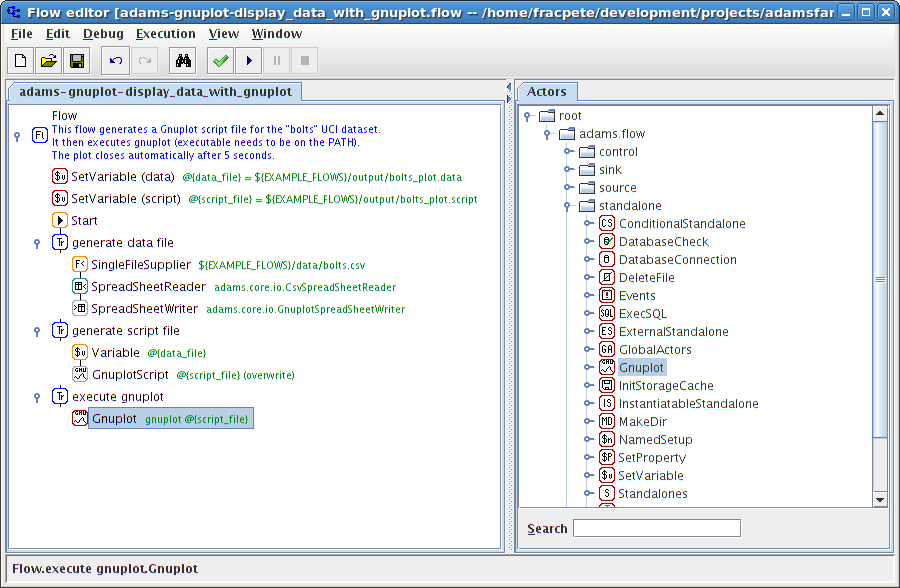
\includegraphics[width=10.0cm]{images/execute_gnuplot.png}
  \caption{Flow that executes Gnuplot with the generated data and script file.}
  \label{execute_gnuplot}
\end{figure}

\textbf{NB:} If the \textit{gnuplot} binary should not be available on the system's path,
you need to specify the full path to it in the \textit{binary} option.


%%%%%%%%%%%%%%%%%%%%%%%%%%%%%%%%%%%
\chapter{Spreadsheets}
ADAMS allows you to load Gnuplot data files as spreadsheet objects and also 
save spreadsheet objects as Gnuplot data files again.
\begin{tight_itemize}
	\item \textbf{read} -- use the \textit{adams.data.io.input.GnuplotSpreadSheetReader}
	class in conjunction with the \textit{SpreadSheetFileReader} transformer.
	\item \textbf{write} -- use the \textit{adams.data.io.output.GnuplotSpreadSheetWriter}
	class in conjunction with the \textit{SpreadSheetFileWriter} sink.
\end{tight_itemize}


%%%%%%%%%%%%%%%%%%%%%%%%%%%%%%%%%%%
% Copyright (c) 2009-2012 by the University of Waikato, Hamilton, NZ. 
% This work is made available under the terms of the 
% Creative Commons Attribution-ShareAlike 4.0 license,
% http://creativecommons.org/licenses/by-sa/4.0/.
%
% Version: $Revision$

\begin{thebibliography}{999}
	% to make the bibliography appear in the TOC
	\addcontentsline{toc}{chapter}{Bibliography}

    % references
	\bibitem{adams}
		\textit{ADAMS} -- Advanced Data mining and Machine learning System \\
		\url{https://adams.cms.waikato.ac.nz/}{}

	\bibitem{esrigrid}
	 	\textit{Esri Grid} -- a raster GIS file format deveoped by Esri. \\
		\url{https://en.wikipedia.org/wiki/Esri\_grid}{}

	\bibitem{kml}
	 	\textit{Keyhole Markup Language} -- an XML notation for expressing
	 	geographic annotation and visualization within Internet-based,
	 	two-dimensional maps and three-dimensional Earth browsers. \\
		\url{http://en.wikipedia.org/wiki/Keyhole\_Markup\_Language}{}

	\bibitem{postgresql}
	 	\textit{PostgreSQL} -- a powerful, open source object-relational
	 	database system. \\
		\url{http://www.postgresql.org/}{}

	\bibitem{postgis}
		\textit{PostGIS} -- a spatial database extender for PostgreSQL
		object-relational database. It adds support for geographic
		objects allowing location queries to be run in SQL.  \\
		\url{http://postgis.net/}{}

	\bibitem{srid4269}
	 	\textit{SRID 4269} -- or NAD 83 (North American Datum). \\
		\url{http://spatialreference.org/ref/epsg/4269/}{}

	\bibitem{mysql}
		\textit{MySQL} -- an open-source relational database management
		system (RDBMS) \\
		\url{http://www.mysql.com/}{}

\end{thebibliography}


\end{document}
